
\chapter{基于图像树木轻量化建模的若干算法}
\label{cha:algorithm}
%----------------------------------PyrLK--------------------------------------
\section{基于改进的PyrLK光流法的特征点匹配方法}
\label{sec:pyrlk}
基于图像的树木建模第一步是三维重建,而三维重建的第一步则是特征点的匹配。
所谓的特征点匹配,是在多张图片中找到空间同一个点在其上的投影位置,从而为三维
重建的后续步骤提供数据支持。这里的特征点,本文选择了具有平移和旋转不变性的
Harris角点,以便用已有的方法快速找出图片中的特殊位置点。然后再结
合改进的PyrLK光流法,对找到的Harris角点进行3D匹配,这里的匹配不只是一般地
基于邻域平移假设的匹配,而是支持平面仿射变换假设的匹配,并且对在容错区间以外
的匹配结果进行了剔除,保证了匹配的精确性和可信度。最后本文将匹配的结果存储到
匹配文件以供后续使用。

%\subsection{对于SIFT特征点匹配的尝试}
%对于特征点的匹配,本文首先尝试的是利用VisualSFM工具自带的SIFT特征点匹配。
%但是经过大量实验发现,该工具自带的SIFT特征点匹配并不能很完整地找到匹配的
%点对,从而导致了三维重建所依赖的数据不足、不精确,最后重建出来一个缺失度
%很大的模型,这样的模型显然不能成功的进行骨架抽取。
%
%根据实验结果分析,除开

\subsection{光流法简介}
光流的概念最早是由James Gibson提出的。1981年,Horn和Schunck创造性地将二维速度
场和灰度联系起来,提出了一种有效的光流计算方法\cite{horn}。基于亮度不变的假设,
图像灰度分布的变化由背景或目标的运动引起,背景或目标的灰度不随时间变化。在这种
假设中,光流法通过目标和背景的不同速度来检测运动目标。

进一步说,将三维空间中的目标和场景对应于二维图像平面运动时,他们在二维图像平
面的投影就形成了运动,这种运动以图像平面亮度模式表现出来的流动就称为光流(Optical Flow)。
也就是说,光流是空间运动物体在观测成像面上对应像素点运动的瞬时速度,这个速度在
图像中以每秒像素点的位移个数来衡量,它巧妙地运用2D的灰度变化来表征3D物体的位置和
结构变化。而光流场(Optical Flow Field)就是所有光流点的集合,是一个2D瞬时速度场。
光流场能够表征整个图像的位移变化,从而对3D运动目标进行检测和跟踪。

在光流法提出以后,很多学者对其进行了研究和改进,并且它们的方法各具特点,算法性能
和运用场景各异。其中颇具代表性的是Lucas-Kanade局部平滑法(LK光流法)\cite{lk},它用基于
微分的方法,利用时变图像灰度的时空微分来计算速度矢量,并且加以图像平滑处理,来进行
光流跟踪。后来在2000年Jean-Yves又提出的基于图像金字塔实现的LK光流法,称为PyrLK光流法\cite{pyrlk}。

\subsection{PyrLK光流算法}
\label{subsec:pyrlk}
假设图片上的像素点的值函数为$I(x,y,t)$,表示坐标位于$(x,y)$的像素点在时刻$t$的像素值
为$I(x,y,t)$。那么经过$\Delta t$时间后,像素值将变为$I(x+\Delta x,y+\Delta y, t+\Delta t)$。
有如下推导:\\
\[  I(x+\Delta x,y+\Delta y, t+\Delta t)=I(x,y,t) + \frac{\partial I}{\partial x}\Delta x 
		+ \frac{\partial I}{\partial y}\Delta y + \frac{\partial I}{\partial t}\Delta t \]
\begin{displaymath}
	\begin{array}{cc}
		\implies & \frac{\partial I}{\partial x}\Delta x 
		+ \frac{\partial I}{\partial y}\Delta y + \frac{\partial I}{\partial t}\Delta t = 0\\
		\implies & \frac{\partial I}{\partial x}V_x 
		+ \frac{\partial I}{\partial y}V_y + \frac{\partial I}{\partial t} = 0 
	\end{array}
\end{displaymath}
\begin{equation}\label{eq:opticalflow}
	\begin{array}{cc}
				\implies & I_xV_x + I_yV_y = -I_t
	\end{array}
\end{equation}

Lucas-Kanade光流法算法基于以上原理,并假设两帧图像之间发生的位移是微量的,而且在一个
点的邻域内这个位移量是常数。这样可以对一个以$p$点为中心的窗口内的像素点写出一个光流方程
组,表征局部图像的运动向量$(V_x,V_y)$需要满足以下方程组:\\
\begin{equation}
	\left\{
		\begin{array}{c}
			I_x(q_1)V_x + I_y(q_1)V_y = -I_t(q_1)\\
			I_x(q_2)V_x + I_y(q_2)V_y = -I_t(q_2)\\
			\vdots\\
			I_x(q_n)V_x + I_y(q_n)V_y = -I_t(q_n)\\
		\end{array}
	\right.
\end{equation}

这里的$q_1,q_2,...,q_n$是局部窗口内的点,$I_x(q_i),I_y(q_i),I_z(q_i)$是图片$I$对$x,y,t$的
偏导函数在$q_i$处的值。将其写为矩阵形式得:\\
\begin{equation}
	A=	
	\left(
	\begin{array}{cc}
		I_x(q_1) & I_y(q_1)\\
		I_x(q_2) & I_y(q_2)\\
		  \vdots & \vdots\\
		I_x(q_n) & I_y(q_n)
		\end{array}
	\right),\quad
	v=
	\left(
	\begin{array}{c}
		V_x\\
		V_y
	\end{array}
	\right),\quad
	b=
	\left(
	\begin{array}{c}
		-I_t(q_1)\\
		-I_t(q_2)\\
		\vdots\\
		-I_t(q_n)
	\end{array}
	\right)
\end{equation}

这个方程组的方程个数远远多于未知数,所以$A$是过约束的,LK光流法运用最小二乘法来求解
出其光流速度。最小二乘法可以参考\ref{subsec:leastsquares}或查阅相关资料。

LK光流法虽然比较直观,但是存在一个问题,由于能够探测到的运动块的大小和所选窗口的大小呈正相关,为了
能够捕捉到大像素块的运动,需要将窗口大小相应调大。但是窗口大小越大,速度就需要在越大的邻域内保持稳定,
就越不符合光流在小范围内稳定的假设。基于金字塔的LK光流法是Lucas-Kanada方法的一种改进版实现,它解决了
窗口大小的与大块运动捕捉的矛盾。其具体思想如下:

设$I$和$J$是两张灰度图片,$I(x)$和$J(x)$分别表示图片$I$和$J$在位置$(x,y)$处的灰度值。现
考虑图片$I$上的一点$\mathbf{u}=(u_x, u_y)$,特征追踪的目标就是找到图片J上的一点$\mathbf{v}
=\mathbf{u}+\mathbf{d}=(u_x+d_x,u_y+d_y)$,使得$I(\mathbf{u})$和$J(\mathbf{v})$“相似”。其中
向量$\mathbf{d}=(d_x,d_y)$表示图片在点$\mathbf{x}$处的光流速度。下面来定义基于邻域的相似,
设$\omega_x$和$\omega_y$是两个整数,将使得下面式子最小化的向量$\mathbf{d}$定义为光流速度:\\
\begin{equation}\label{eq:similarity}
	\epsilon(\mathbf{d})=\epsilon(d_x,d_y)=\sum_{x=u_x-\omega_x}^{u_x+\omega_x}\sum_{y=u_y-\omega_y}
	^{u_y+\omega_y}(I(x,y) - J(x+d_x,y+d_y))^2.
\end{equation}
其中邻域窗口大小为$(2\omega_x+1)\times(2\omega_y+1)$。式子的含义为寻找向量$\mathbf{d}$使得
$\mathbf{u}$和$\mathbf{v}$在邻域窗口大小内的差异最小化。

然后该方法将图像金字塔化,即将原图像作为最高分辨率层,逐步降低图像的分辨率,并作为新的一层,加入到
LK光流法的迭代序列。通过这样多分辨率图层,使得邻域窗口的大小在低分辨率图像对应的区域可以映射到高
分辨率图像的更大的像素区域,从而支持了大块运动。

\subsection{PyrLK光流算法的改进}
\label{subsec:revisedpyrlk}
\subsubsection{加入仿射变换}
对于PyrLK光流算法,已经能够很好的解决几乎任何像素块大小由平移主导的匹配。然而,这并不足以完美地
解决树木上点的匹配问题。因为相邻的两帧图像要求在空间形成一定的夹角进行拍摄,这样在两帧图像上,
也一定会产生由空间旋转投影过后带来的平面旋转。而这样的变换在PyrLK光流算法里是无法解决的,因为PyrLK
只是简单的将点的匹配依赖于点的平移。所以,有必要对PyrLK光流算法进行由平移变换到放射变换的扩展。

假设两个点的匹配满足仿射矩阵$A$,那么有:\\
\begin{equation}
	\left(
	\begin{array}{c}
		\Delta x'\\
		\Delta y'\\
		0
	\end{array}
	\right)
	=
	\left(
	\begin{array}{ccc}
		a_{11} & a_{12} & a_{13}\\
		a_{21} & a_{22} & a_{23}\\
				0 & 0 & 0
	\end{array}
	\right)
	\cdot
	\left(
	\begin{array}{c}
		\Delta x\\
		\Delta y\\
		1
	\end{array}
	\right)
\end{equation}
将其代入式\ref{eq:opticalflow}得:\\
\begin{equation}
	(a_{11}\ a_{12}\ a_{13}\ a_{21}\ a_{22}\ a_{23})\cdot
	\left(
	\begin{array}{c}
		\frac{\partial I}{\partial x}\Delta x\\
        \frac{\partial I}{\partial x}\Delta y\\
        \frac{\partial I}{\partial x}\\
        \frac{\partial I}{\partial y}\Delta x\\
        \frac{\partial I}{\partial y}\Delta y\\
        \frac{\partial I}{\partial y}\\
	\end{array}
	\right)
	=-I_t
\end{equation}

运用最小二乘法可以得到$A$的解。

将PyrLK中的定义式\ref{eq:similarity}稍作修改可可使得其支持仿射变换:\\
\[ Let\quad \mathbf{a_1}=(a_{11},a_{12},a_{13})\quad \mathbf{a_2}=(a_{21},a_{22},a_{23})\quad
\mathbf{b}=(d_x,d_y,1)\]\\
\begin{equation}\label{eq:affine}
	\epsilon(\mathbf{d})=\epsilon(d_x,d_y)=\sum_{x=u_x-\omega_x}^{u_x+\omega_x}\sum_{y=u_y-\omega_y}
	^{u_y+\omega_y}(I(x,y) - J(x+\mathbf{a_1}\cdot \mathbf{b},y+\mathbf{a_2}\cdot \mathbf{b}))^2.
\end{equation}


\subsubsection{反向追踪与中值过滤以提高鲁棒性}
本文前面几个小节一直在探讨如何改进和完善匹配的方法,从而提高精度和匹配可信度。然而,
这其中有一个问题,单方向的去追踪匹配点是否就能确定该两个匹配点真正的匹配呢?其实不然,
要确定两个点完全符合之前算法描述的特点,还需要反向进行检查,看$\mathbf{u}$和$\mathbf{v}$之间
的匹配是否是双向和可逆的。换句话说,本文之前定义的“相似”其实是单方面的$\mathbf{u}$相似于
$\mathbf{v}$,而$\mathbf{v}$是否相似于$\mathbf{u}$还不得而知。因此,考虑到算法的完整性和鲁棒性,
有必要进行反向的匹配来确定它们完全匹配。或者退一步,给出一个容错的区间,定义当差异度小于阈值
时,两个点“相似”。基于此出发点,本文提出了基于反向追踪来对匹配对进行验证的思想。

另外,对于任何的匹配算法,不可能真正地达到完美和全部匹配。所以对于用金字塔LK光流法进行匹配过后,
应该进行一定地筛选措施,以除去一些“边缘化”的匹配,使得所有匹配对都能有更高的可信度,而不是完全
依赖于算法的实际表现情况。本文提出了基于中值过滤的筛选方法,该方法将对两个步骤进行中值滤值:\\
\begin{itemize}
	\item \textbf{邻域相似度中值过滤}: 在实施过光流算法以后,对于每两个匹配的点,计算其归一化相关系数,作为其相似度。归一化相关
		系数的计算式如下:
		\begin{equation} \label{eq:ccoeff}
			R(x,y) = \frac{\sum_{x',y'}(T'(x',y')\cdot I'(x + x', y + y'))}
			{\sqrt{\sum_{x', y'}T'(x',y')^2\cdot \sum_{x',y'}I'(x+x',y+y')^2}}
		\end{equation}
		然后计算所有匹配对的相似度中值,对于低于这个中值的点对,本文将
		视其为不满足可信度的点对而剔除掉。
	\item \textbf{反向追踪差异度中值过滤}: 在进行反向追踪过后,每个点对将得到一个差异值,表示从后一帧图片的点到
		反向追踪得到的点与前一帧图像的对应点的空间位置差。本文对于反向追踪差异度低于中值的点对进行剔除,
		视其为不满足可信度的点对。
\end{itemize}

经过反向追踪和中值过滤还剩下的匹配点对,本文视为可信的匹配点对,该步骤对于提高算法的鲁棒性尤为
重要。算法\ref{alg:backtrack}给出了反向追踪和中值过滤的伪代码:\\
\begin{algorithm}[H]
	\caption{反向追踪\&中值过滤}
	\label{alg:backtrack}
	\begin{algorithmic}[1]
	\Require 反向追踪差异度数组$\mathbb{B}[1..n]$,邻域相似度数组$\mathbb{S}[1..n]$
	\Require 源匹配点对数组$\mathbb{P}$
	\Ensure 过滤后匹配点对数组$\mathbb{Q}$
	\State 初始化反向追踪差异度中值mb,邻域相似度中值ms
	\State SortArray($\mathbb{B}[1..n]$)
	\State SortArray($\mathbb{S}[1..n]$)
	\State $mid=(n+1)/2$
	\State $mb=\mathbb{B}[mid],\quad ms=\mathbb{S}[mid]$
	\For{$i=1$ to $n$}
	\If{$\mathbb{B}[i] < mb \cap \mathbb{S}[i] > ms$}
		\State $\mathbb{Q}.AddMatch(\mathbb{P}[i])$
	\EndIf
	\EndFor
	\State \Return $\mathbb{Q}$
	\end{algorithmic}
\end{algorithm}

\subsection{支持仿射变换和提高鲁棒性的的PyrLK光流法}
经过仿射变换支持和提高鲁棒性的PyrLK光流法比起传统的PyrLK光流法,其适应性和稳定性都有
大大的提升。其主要表现在:\\
\begin{itemize}
	\item \textbf{对旋转的支持}: 加入了仿射变换意味着新的匹配算法能够很好的适应从三维场景
		旋转而投影形成的二维的旋转,而本文对树木的拍摄每一帧都是在上一帧的基础上进行三维的
		空间旋转,所以对旋转的支持可以大大提升匹配的准确性。
	\item \textbf{匹配验证}: 对于每一对匹配点,本文运用归一化相关系数对它们的邻域的相似性
		做进一步验证,只有通过相似匹配验证的点对,本文才认为是真正相似的点对。
	\item \textbf{剔除不稳定匹配}: 单方向的匹配不能确认两个点真正的匹配,所以本文的反向追踪
		可以对匹配进行双向的确认,从而剔除不满足反向追踪匹配的点对。以进一步提高算法的鲁棒性。
\end{itemize}

图\ref{fig:pyrlk}展示了传统的PyrLK光流法与本文的改进版本的对比。这里的图片用了不同的颜色通道来表示,
其中绿色通道代表源图片,紫色通道代表目的图片,用红色的线段表示图片间点的匹配关系。从图\ref{fig:pyrlk}(a)中可以发现,
传统的PyrLK光流算法几乎没有任何的验证措施,所以导致其出现了大量的错误匹配。比如图中远处的树林,
由于其离观察原点比较远,所以视角的转动会导致其运动位移较大,然而图\ref{fig:pyrlk}(a)中所示远处森里的光流值并不大,还有图中
近处的树木样本的匹配也非常不准确,有相当一部分点匹配到了背景上面去,这必然会使重建过程中由于错误信息
而重建出错误的点云。而图\ref{fig:pyrlk}(b)总,无论是远处大位移的树林还是近处的树木
枝条,光流值的大小都比较合适,而且匹配度是相当高的。可见改进版本比传统版本对于树木特征点的匹配有明显的提高,
由于图片特征点匹配是重建步骤中的第一步,所以准确和稳定的匹配对于后期的重建工作至关重要,它将使得后期的工作事半功倍。
\begin{figure}[H]
	\centering
	\subfloat[传统PyrLK光流法]{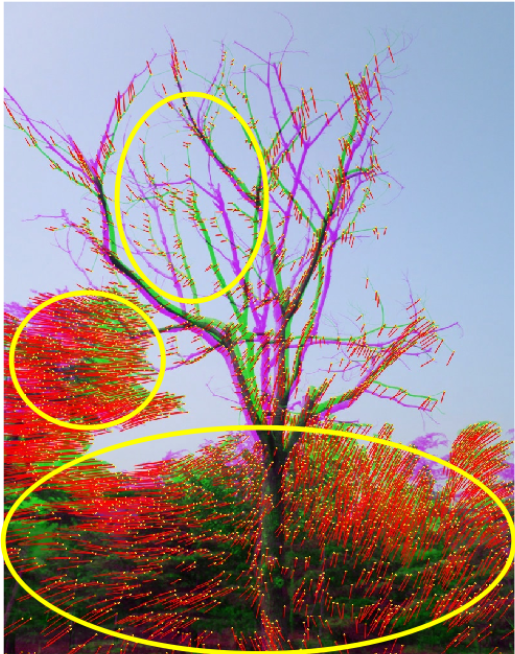
\includegraphics[height=10cm]{old.png}}\hspace{4em}
	\subfloat[改进的PyrLK光流法]{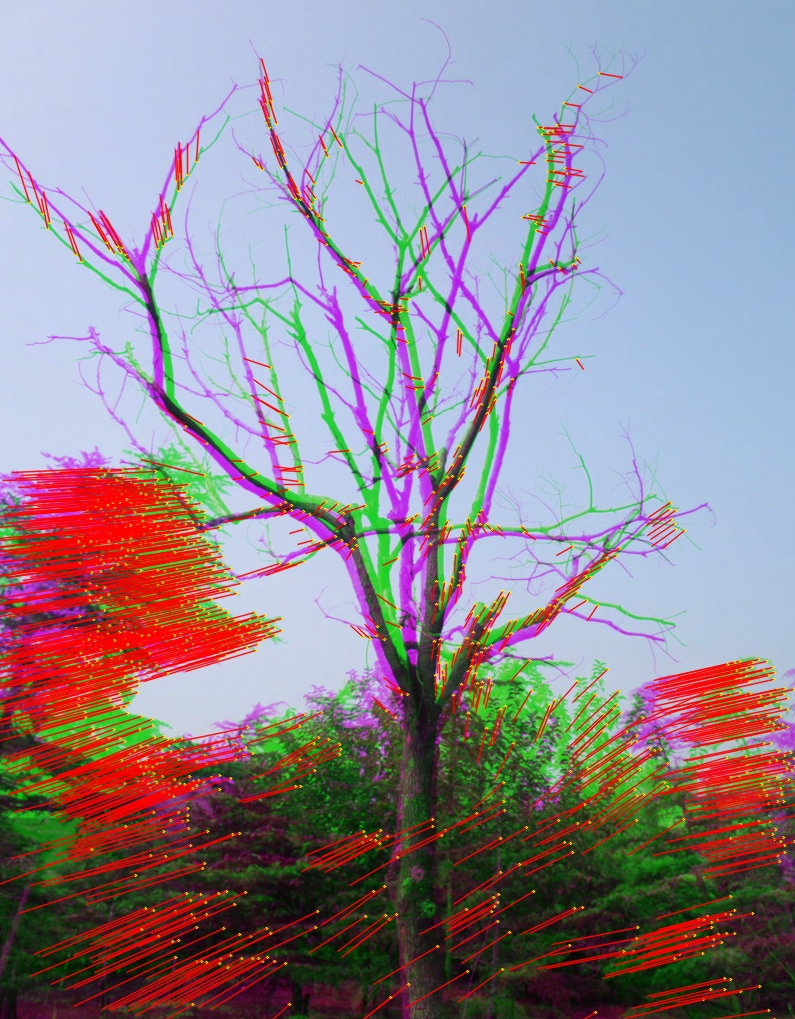
\includegraphics[height=10cm]{new.png}}
	\caption{支持仿射变换和提高鲁棒性的PyrLK光流法与传统光流法对比图}
	\label{fig:pyrlk}
\end{figure}


\clearpage
算法\ref{alg:pyrlk}给出了经过添加仿射变换支持和提高鲁棒性的PyrLK光流法算法的伪代码:\\
\begin{algorithm}[H]
	\caption{支持仿射变换和容错机制的PyrLK光流法}
	\label{alg:pyrlk}
	\begin{algorithmic}[1]
		\Require 图像$I$,$J$,图像$I$中的点$\mathbf{u}$
		\Ensure 图像$J$中对应点$\mathbf{v}$
		\State 构建图像$I$和$J$的金字塔表示: $\{I^L\}_{L=0,...,L_m}$和$\{J^L\}_{L=0,...,L_m}$
		\State 初始化金字塔估计值: $g^{L_{m}}=(g_x^{L_m}, g_y^{L_m})=(0,0)$
		\For{$L=L_m$to 0 with step of -1}
		\State 定位图像$I^L$上的点$\mathbf{u^L}$: $\mathbf{u}^L=(u_x,u_y)=\mathbf{u}/2^L$
		\State 设$\mathbf{a_1}=(a_{11},a_{12},a_{13})\quad \mathbf{a_2}=(a_{21},a_{22},a_{23})\quad 
				\mathbf{b}=(d_x^L, d_y^L, 1$
		\State 定义相似度:
				\[ \epsilon(\mathbf{d^L})=\epsilon(d_x,d_y)=\sum_{x=u_x-\omega_x}^{u_x+\omega_x}\sum_{y=u_y-\omega_y}
				^{u_y+\omega_y}(I(x,y) - J(x+\mathbf{a_1}\cdot \mathbf{b},y+\mathbf{a_2}\cdot \mathbf{b}))^2.\]
				\State 最小二乘法估计出$d^L$,使得$\epsilon $达到最小值
		\State L-1层金字塔估计值: $g^{L-1}=2(g^L+d^L)$
		\EndFor
		\State 最终光流向量: $\mathbf{d}=\mathbf{g^0}+\mathbf{d^0}$
		\State $\mathbf{v}=\mathbf{u+d}$
		\If{BackwardTrack$(\mathbf{v})$ = true}
			\If{MedianFilter$(\mathbf{v})$ = true}
				\State \Return $\mathbf{v}$
			\Else
				\State \Return NULL
			\EndIf
		\Else
			\State \Return NULL
		\EndIf
	\end{algorithmic}
\end{algorithm}

%---------------------------------三维重建-----------------------------------
%\section{基于体素泛洪与空间反向投影的三维重建}
%\label{sec:3drec}

%---------------------------------骨架抽取-----------------------------------
\clearpage
\section{基于三维体素泛洪与线性拟合的三维树木骨架抽取}
\label{sec:sklextract}
在获取了精确的点云模型之后,出于后续轻量化的考虑,需要将模型的存储方式由
密集的点云转化为逻辑的父子结构。用树形的数据结构来表达现实的树结构,这是很
自然的想法,相对于面片结构,树形结构也是一种更为轻量化的存储方式。每个节点表示
树枝的起点,存储着该节点的空间位置,半径和该节点的父子枝信息以及兄弟信息。一个
节点和它的一个子节点形成一个空间线段,若干空间线段组成一条连续的树枝。

本文从树的生长规律入手,从根节点往子节点生长。生长的依据则为当前节点所在邻域
内的空间点云分布,节点邻域大小由步长来控制,步长会探索式地递增,直到达到了增长的阈值,
邻域大小才确定下来。然后从其点云分布拟合出各个分支的方向,从而生长出新的子节点,
并递归地生长下去直到点云的边界。

\subsection{三维体素模型}
前面三维重建步骤得到的结果是一个点云模型,该模型中的点数量庞大,不适于后续的
邻域搜索,因此我们需要对点云进行体素化处理。所谓体素化,就是将点云占据的空间
划分成一个个的小立方体,每一个立方体称之为一个体素。

在将点云模型转化为体素模型以后,对于点云的邻域搜索便转化为了对于空间临近体素的
搜索,体素的位置就反映了点集的位置,因此不用每次搜索都遍历整个点云,而是只用将
步长范围体素中的点集遍历即可。由于体素是我们处理的基本单位,所以体素的大小也
直接决定了体素模型的精度,因此,在确保非空体素的空间连续性和效率允许的基础上,
本文建议让体素尽可能的小,以保证模型的精度。将点云模型转换为体素模型的伪代码
在算法\ref{alg:voxel}中给出。图\ref{fig:voxel}形象地展示了将空间体素化以后树木的点云模型
在体素块中的分布情况。

\begin{figure}[H]
	\centering
	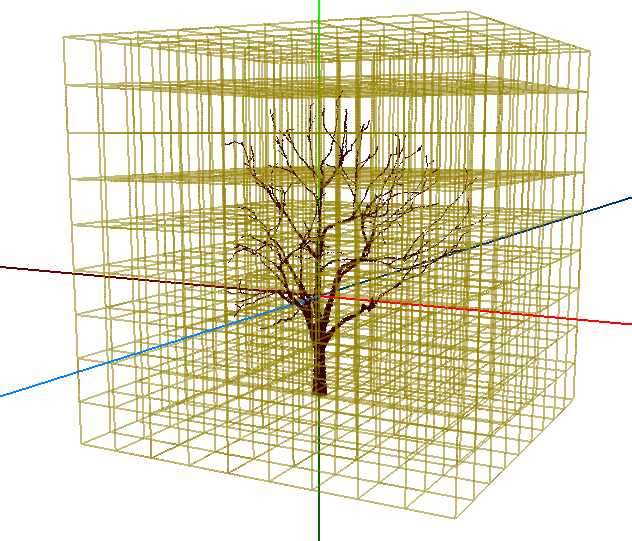
\includegraphics[height=8cm]{voxel.png}
	\caption{三维体素模型}
	\label{fig:voxel}
\end{figure}

\begin{algorithm}[H]
	\caption{点云模型体素化}
	\label{alg:voxel}
	\begin{algorithmic}[1] 
	\Require 点云模型$M$
	\Require 体素维度$d$
	\Ensure 三维体素数组$\mathbb{V}[1..d,1..d,1..d]$
	\State 初始化点云边界值$X_{max}=Y_{max}=Z_{max}=MIN\uline\quad FLOAT,X_{min}=Y_{min}=Z_{min}=MAX\uline\quad FLOAT$
	\ForAll{空间点$P(P_x,P_y,P_z) \in M$}
		\State $CheckBoundary(P)$
	\EndFor
\ForAll{空间点$P(P_x,P_y,P_z) \in M$}
\State $V_x = \frac{P_x-X_{min}}{X_{max}-X_{min}}\cdot d$
\State $V_y = \frac{P_y-Y_{min}}{Y_{max}-Y_{min}}\cdot d$
\State $V_z = \frac{P_z-Z_{min}}{Z_{max}-Z_{min}}\cdot d$
\State $\mathbb{V}[V_x, V_y, V_z] = \mathbb{V}[V_x, V_y, V_z] \bigcup \{P\} $
	\EndFor
\end{algorithmic}
\end{algorithm}

\subsection{三维体素泛洪确定邻域范围}
在确定了三维体素模型以后,便需要从根到叶,自底向上地对树的骨架结构进行生长。
生长的依据是已经得到的体素模型,将体素模型中点的分布作用于骨架的分支,便可以
张成骨架模型。

具体方法是将根节点置为当前节点,对其进行三维泛洪,首先对其相邻的27个体素进行泛洪,若
体素不为空,则将其加入邻域范围,若为空,则停止向该方向进行迭代。同时将加入邻域
范围的体素置为无效,表示其已经参与了泛洪,不再参与骨架的重建,这样不仅可以对算法
的结束有一个很好的约束条件,同时也可以减少重复处理的次数,加快算法的完成。然后进行下一次迭代,
对新加入的体素进行27方向的泛洪,并把有效的体素加入到邻域范围。接着比较两次迭代
体素增加的比例,如果低于设置的阈值,则停止迭代,当前的邻域范围即为三维泛洪得到
的当前节点的邻域范围。

图\ref{fig:3dfld}展示了三维体素泛洪确定邻域的步骤。\ref{fig:3dfld}(a)为其初始状态,
即邻域范围为当前体素。其中橙色的区域表示邻域范围,蓝色的区域表示未探索区域,灰色区域
表示空的体素,而绿色区域表示已经在之前的枝干邻域。\ref{fig:3dfld}(b)表示体素泛洪经过
一次迭代以后的状态,因为体素泛洪只会对与当前邻域范围相邻的未探索区域(蓝色方块)进行扩展,
所以\ref{fig:3dfld}(a)只会向黄色箭头指向的体素进行扩展,从而得到\ref{fig:3dfld}(b)。在得到
新的邻域后,首先会计算所新增的点的数量与之前的数量的比值有没有低于阈值,如果低于阈值,则停止
邻域的扩张。最后将得到\ref{fig:3dfld}(c)中的邻域范围。

\begin{figure}[H]
	\centering
	\subfloat[初始状态(邻域范围为1个体素)]{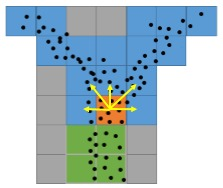
\includegraphics[height=3cm]{fld1.jpg}}\hspace{4em}
	\subfloat[第一次泛洪迭代(邻域范围为6个体素)]{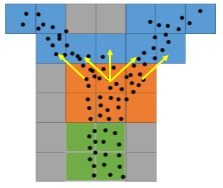
\includegraphics[height=3cm]{fld2.jpg}}\hspace{4em}
	\subfloat[第二次泛洪迭代(邻域范围为11个体素)]{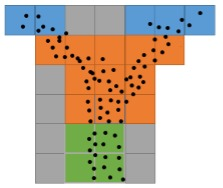
\includegraphics[height=3cm]{fld3.jpg}}
	\caption{体素泛洪示意图}
	\label{fig:3dfld}
\end{figure}

三维体素泛洪确定邻域范围算法的伪代码在算法\ref{alg:3dfld}中给出。
\begin{algorithm}[H] 
	\caption{三维体素泛洪确定邻域范围}
	\label{alg:3dfld}
	\begin{algorithmic}[1]
		\Require 当前体素$C$,三维体素数组$\mathbb{V}[1..d,1..d,1..d]$,
		泛洪方向数组$\mathbb{D}[1..27]$,邻域范围增长比例阈值$\lambda$
		%\Require 三维体素数组$\mathbb{V}[1..d,1..d,1..d]$
		%\Require 泛洪方向数组$\mathbb{D}[1..27]$
		%\Require 邻域范围增长比例阈值$\lambda$
		\Ensure	邻域范围内体素集合$\mathbb{S}$
		\State 初始化单次迭代新增体素集合$\mathbb{S'}$
		\State $\mathbb{S'}.AddVoxel($根节点所在体素$)$
		\ForAll{泛洪方向$Direction \in \mathbb{D}$}
			\State $NewIndex = C.Index + Direction$
			\State $NewVoxel = \mathbb{V}[NewIndex.x,NewIndex.y,NewIndex.z]$
			\If{$NewVoxel$非空$\bigcap NewVoxel$有效}
				\State $\mathbb{S'}.AddVoxel(NewVoxel)$
			\EndIf
		\EndFor
		\State 体素增长比例$\mu=\frac{\mathbb{S'}.VoxelCount}{\mathbb{S}.VoxelCount}$
		\If{$\mu > \lambda$}
			\ForAll{$voxel \in \mathbb{S'}$}
				\State 把$voxel$作为当前体素进行递归调用
			\EndFor
		\EndIf
		\State \Return $\mathbb{S}$
	\end{algorithmic}
\end{algorithm}

在进行三维泛洪的时候,可以编程实现27个方向迭代过程的并行化,以提高算法的效率。

\subsection{通过最小二乘法线性拟合确定分支方向}
\label{subsec:leastsquares}
当得到邻域范围以后,便得到了邻域内体素在基于当前节点27个方向上的密度分布,而
每个体素内又包含着若干的点,因此等于是得到了在当前节点邻域内的点云分布情况。
接下来的工作就是怎样从各个方向的点云的分布情况抽取出核心的骨架。本文应用线性
拟合的方法来从密集的点中抽取出一条直线,作为该部分的骨架方向。

该方法首先要剔除掉那些点云密度很小的方向,以免每个节点都朝各个方向长出一些
细碎的枝条。因为这些细碎的枝条就算在此步中不剔除,到后续的轻量化的时候也不容许
它们的存在。

然后对于剩下的若干方向$d_1,d_2...d_k$,每个方向都对应着树木的一个骨架。在处理
某个方向$d_i$时,将其包含的体素中的所有点抽取出来,得到一个密集的点集$S_i$。
然后采用待定方程的办法,设直线方程为:
\begin{equation}
	\mathbf{x} = \mathbf{x_0} + \mathbf{d}t,\quad(t \in [0,\infty))
\end{equation}

其中$\mathbf{x_0}$是当前节点的坐标,$\mathbf{d}$是待拟合的直线方向。我们假设
点集$S_i$中的点$P_1,P_2,...P_m$都在直线上,则可以得到以下方程组:\\

\begin{equation} \label{eq:line}
	\left\{ 
		\begin{array}{lll}
			a_{11}d_x+a_{12}d_y+a_{13}d_z & = & b1\\
			a_{21}d_x+a_{22}d_y+a_{23}d_z & = & b2\\
			... & & \\
			a_{n1}d_x+a_{n2}d_y+a_{n3}d_z & = & bn
		\end{array}
	\right.
\end{equation}

其中具体数值未给出,注意这里的$n=3m$,因为每个点$P$可以提供三个方向的方程式。
在这个方程组中,令\\
\begin{displaymath}
	\mathbf{U}=
\left(
\begin{array}{ccc}
	a_{11} & a_{12} & a_{13}\\
	a_{21} & a_{22} & a_{23}\\
	... & ... & ...\\
	a_{n1} & a_{n2} & a_{n3}\\
\end{array}
\right)
,\quad
\mathbf{d}=
\left(
\begin{array}{c}
	d_x\\
	d_y\\
	d_z
\end{array}
\right)
,\quad
\mathbf{b}=
\left(
\begin{array}{c}
	b_1\\
	b_2\\
	...\\
	b_n
\end{array}
\right)
\end{displaymath}


在实践中,由于筛选方向上的点数较多且发散分布,由线性代数的理论知,$\mathbf{U}$是过约束的,
即$n>r$,其中$r$是矩阵$\mathbf{U}$的秩。这种情况下没有标准的解,只能找到使误差最小的向量$\mathbf{d}$,
误差定义为:\\
\begin{equation}
	E\xlongequal{def} \sum_{i=1}^n(\mathbf{d}t_i - \mathbf{x_i} + \mathbf{x_0})^2=|\mathbf{Ud}-\mathbf{b}|^2
\end{equation}

由于$E$正比于方程的均方误差,因此只要E达到最小值,那么点集相对于该直线的波动就最
小。换句话说,也就是该直线最好的模拟了该点集所表示的骨架。由线性代数的方法很容易
可以解得$\mathbf{d}=\mathbf{[(U^TU)^{-1}U^T]b}$。图\ref{fig:fitting}展示了由当前
节点(蓝色节点)分别向两个点云集合拟合出的两条直线(红色线段),这两条直线将被作为两个
分支的方向。从图中可以看出线性拟合的方法可以很好的估计出树木分枝的方向,从而准确的
恢复出树木的父子结构。

\begin{figure}[H]
	\centering
	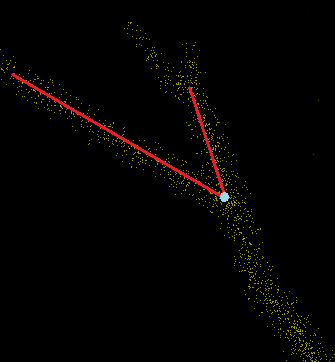
\includegraphics{fitting.png}
	\caption{线性拟合计算分支方向}
	\label{fig:fitting}
\end{figure}

算法\ref{alg:sklextract}给出了得到邻域信息后进行骨架方向抽取的伪代码,其中\textit{Least Squares Processing}表示运用最小二乘法进行
线性拟合。

\begin{algorithm}[H]
	\caption{基于邻域的骨架方向计算}
	\label{alg:sklextract}
	\begin{algorithmic}[1] 
		\Require 当前节点体素$V$
		\Require 骨架方向数组$\mathbb{D}[1..n]$
		\Ensure 当前节点子节点集合$\mathbb{S}$
		\ForAll{骨架方向$d\in D$}
			\State $NewChild\gets Least Squares Processing$
			\State $\mathbb{S}.AddChild(NewChild)$
		\EndFor
		\State \Return $\mathbb{S}$
	\end{algorithmic}
\end{algorithm}

\subsection{获取子枝长度和半径}
树木骨架的长度和半径对树木模型的真实感有着十分显著的贡献,所以尽可能准确的获得子枝的长度和
半径信息能够有助于重建出极具真实感的树木模型。对于树木枝干半径的获取方法有许多,
主要分为根据规则生成半径和从树木点云结构中获取半径两种方式。

对于基于规则来生成半径,最简单的方法是对树木半径进行线性地递减,即$r=cR$,其中
$r$为子枝半径,$R$是父枝半径,$c$为一个线性倍数,这个倍数可以固定,也可以进行
随机的扰动从而增进多样性。Leonardo da Vinci在经过大量观察后总结出了一种更符合自然规律
的树木父子枝直径的关系公式:$D^2=\sum_{i=1}^n{d_i^2}$,其中$D$为父枝直径,$d_i$为第
$i$个子枝的直径,$n$为子枝的数量。这个公式被广泛地用于树木枝干的半径模拟。

区别于基于规则的半径生成方法,本文为了进一步提升真实感,选择在进行子枝方向抽取的同时,
同样进行半径抽取的方法。注意,用该方法的前提是点云分布须均匀化,然而基于图像进行三维重建
得到的树木点云会呈现表皮化的现象,这是由于图片上的点都是树木的表皮点,所以在得到
三维点云后,是需要进行一些修复工作的,本文用随机点填充的方法对该点云模型进行了实心化
的修复。当点云分布满足均匀化时,在对某个骨架进行拟合之后,对于拟合出来的直线,来计算
所有参加拟合该直线的点到该直线的平均距离$D_{avg}$,然后就可以计算该骨架的半径$R=D_{avg}*2$。
由于点云分布均匀,所以半径显然就是平均距离的2倍。该算法的伪代码在算法\ref{alg:radius}中给出。\\

\begin{algorithm}[H]
	\caption{骨架半径抽取}
	\label{alg:radius}
	\begin{algorithmic}[1] 
		\Require 拟合出的当前子枝所在直线$L$
		\Require 当前子枝的点集$\mathbb{S}$
		\Ensure 当前子枝半径$R$
		\State 初始化点到直线距离之和$D_{sum}=0$
		\ForAll{空间点$P \in \mathbb{S}$}
		\State 点到直线距离$D_{sum}+=CalculateDistance(P, L)$
		\EndFor
		\State 平均距离$D_{avg}=D_{sum}/\mathbb{S}.Count$
		\State 子枝半径$R=D_{avg}*2$
		\State \Return $R$
	\end{algorithmic}
\end{algorithm}

图\ref{fig:radius}给出了三种半径求解方法的效果对比。\ref{fig:radius}(a)给出了线性衰减方法
的结果,该方法中子枝半径以父枝半径的线性倍衰减。\ref{fig:radius}(b)给出了前文提到的Leonardo
 da Vinci规则所生成的半径情况。\ref{fig:radius}(c)则采用本文中基于线性拟合直线,再计算所有点
 到该直线平均距离的方法。从三者的效果中可以看出,线性衰减容易出现部分枝条生长不自然的现象,究其
 原因,还是因为一个单一的绝对的线性系数无法适用于所有的枝条,它对于某些枝条会偏大,对于另外一些
 枝条会偏小。 Leonardo规则虽然给出的是一种父子枝之间的相对关系,从一定程度上解决了线性系数单一
 绝对而导致的问题,但是它生成的树木枝干会出现过于均与化,而没有捕捉到现实中树木各个局部的特征。
 本文的方法则由于其基于对所有点的实际恢复坐标进行统计,而更加注重树木的实际局部特征情况,
 其效果也是三者之中最好的。
 \begin{figure}[H]
	\centering
	\subfloat[样本图像]{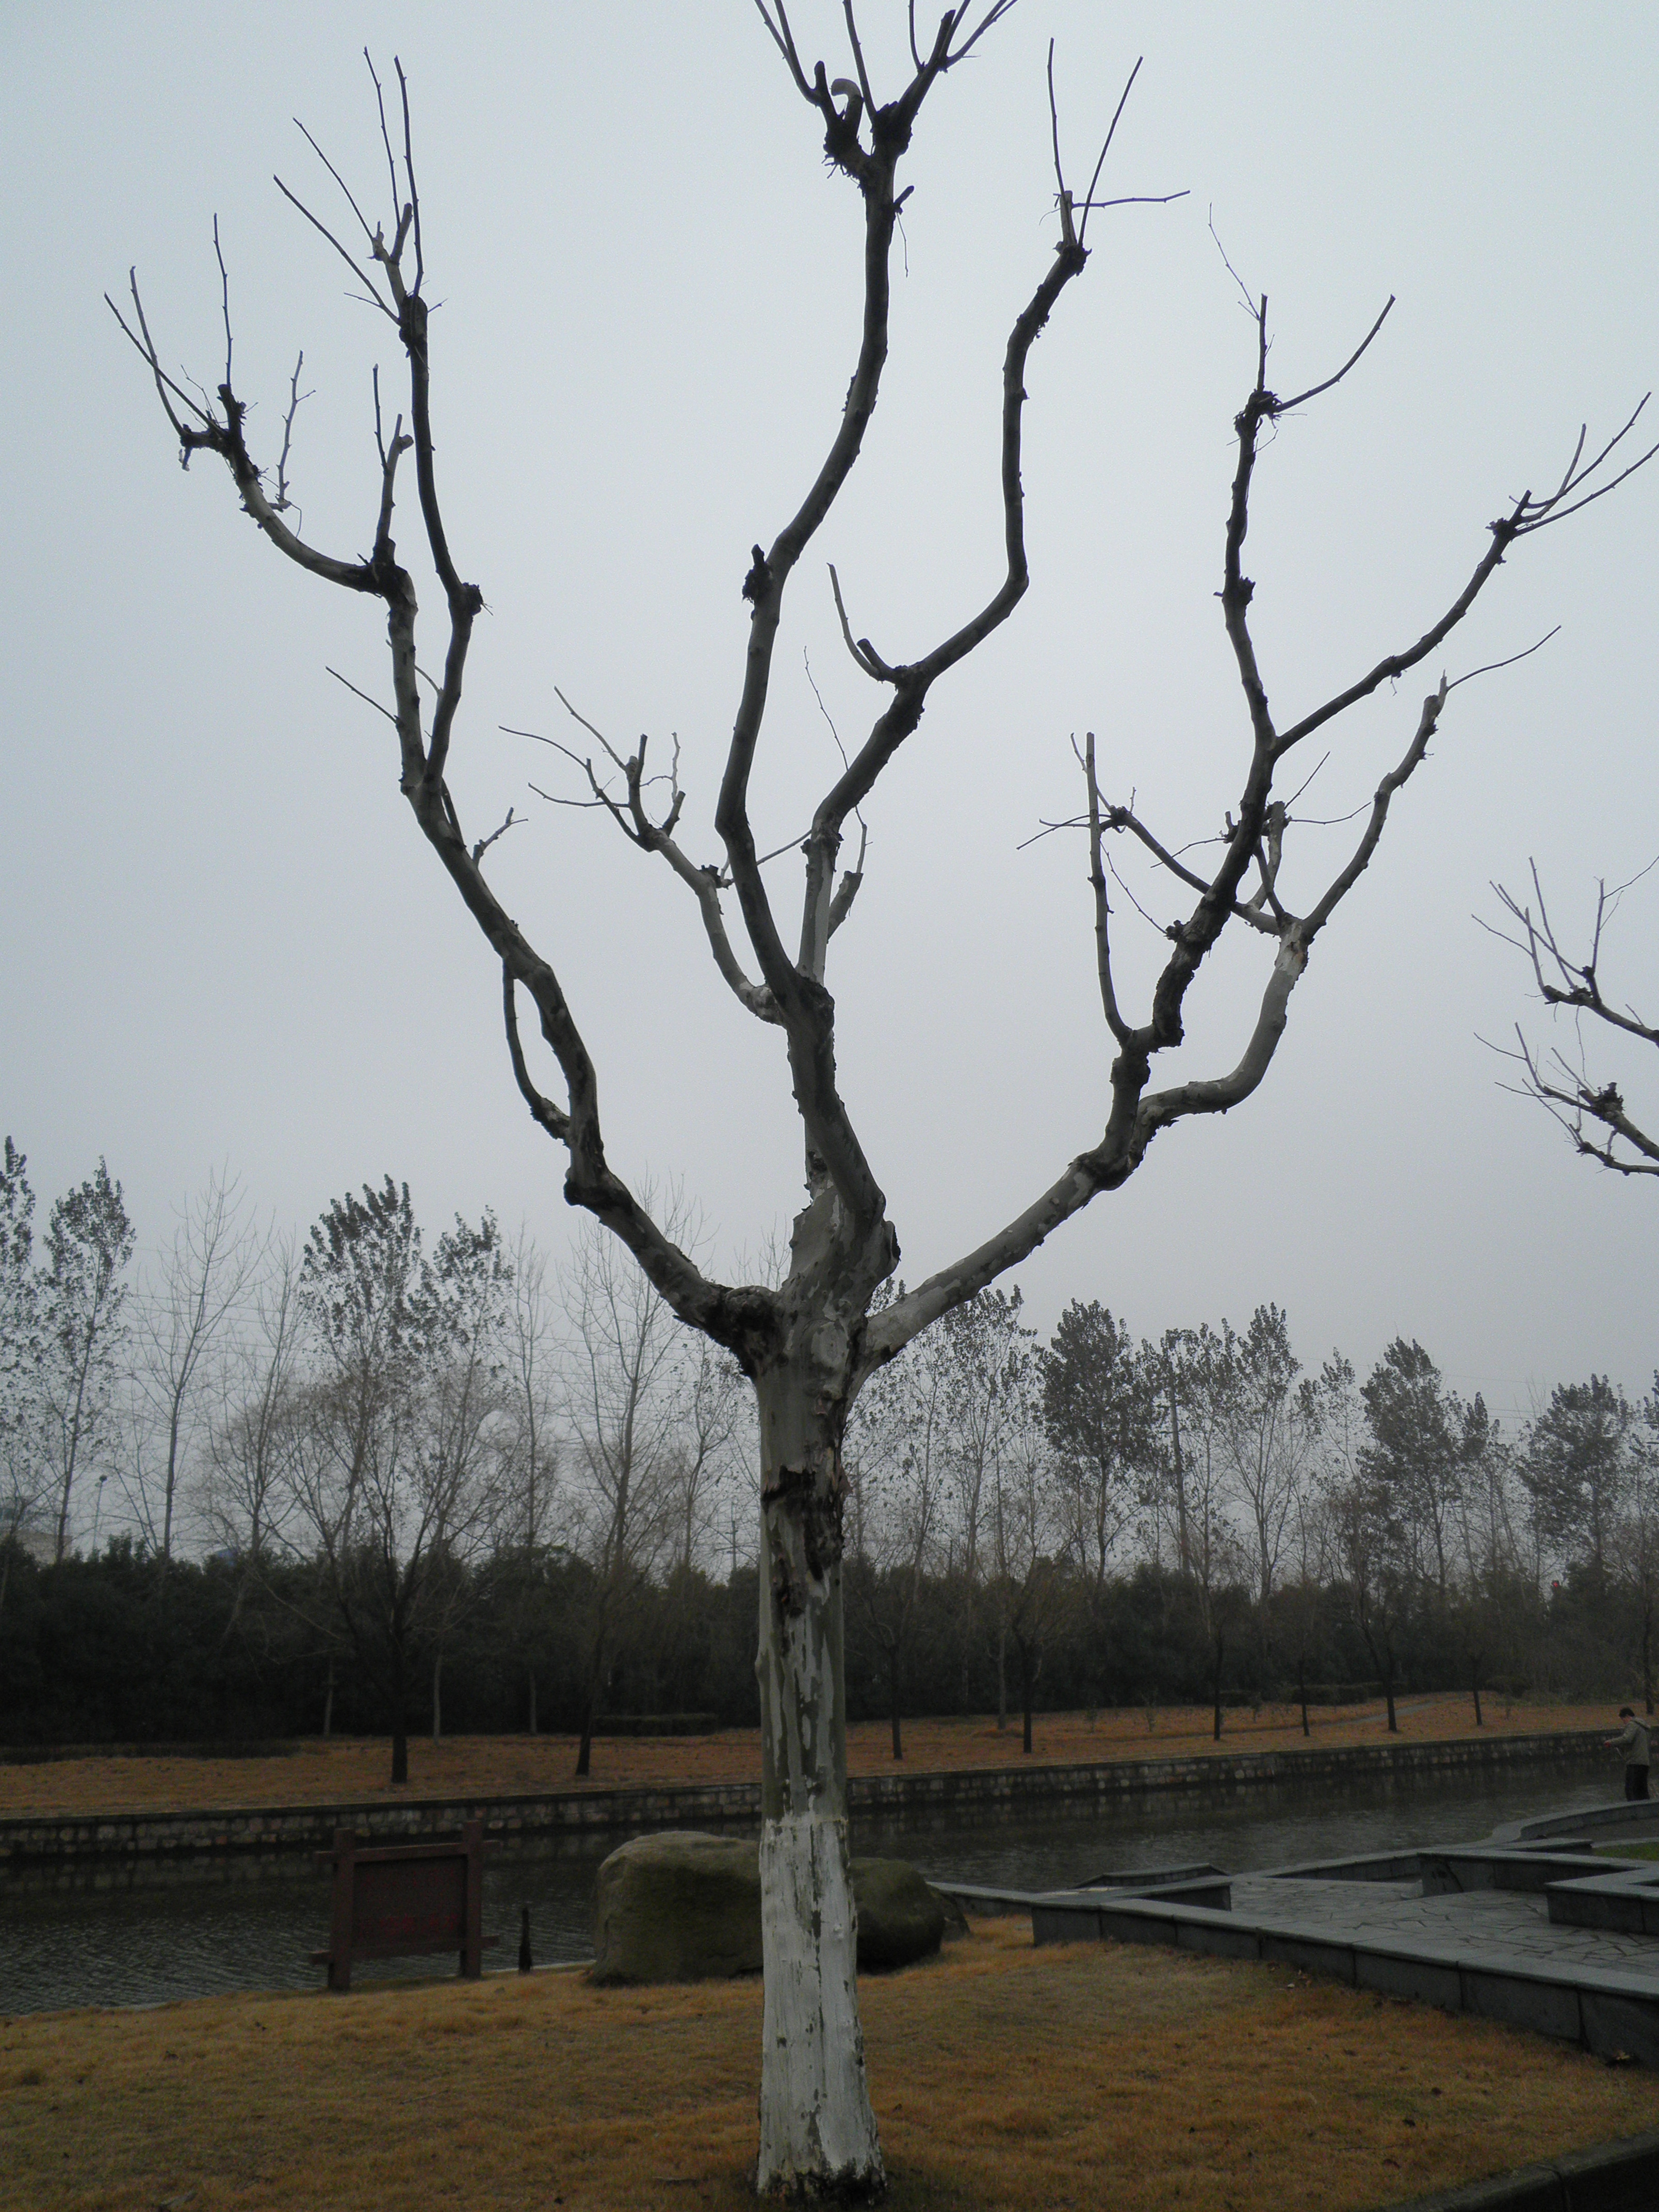
\includegraphics[height=6cm]{rsample.jpg}}\hspace{4em}
	\subfloat[线性衰减]{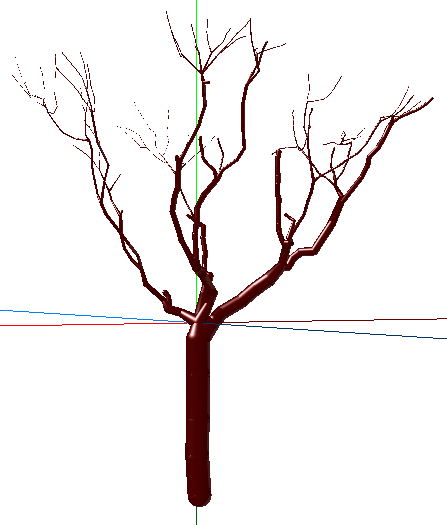
\includegraphics[height=6cm]{rlinear.png}}\hspace{4em}
	\subfloat[Leonardo规则生成]{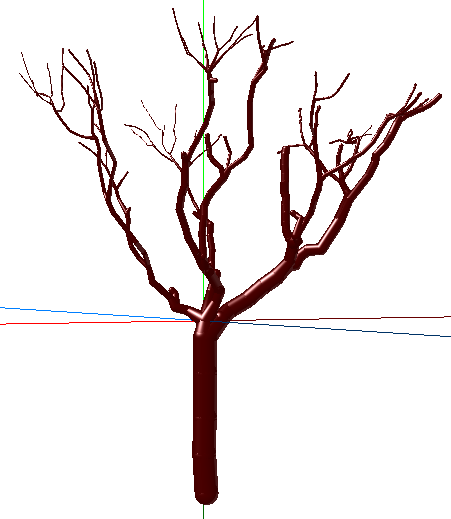
\includegraphics[height=6cm]{rsquare.png}}\hspace{4em}
	\subfloat[基于拟合的半径抽取]{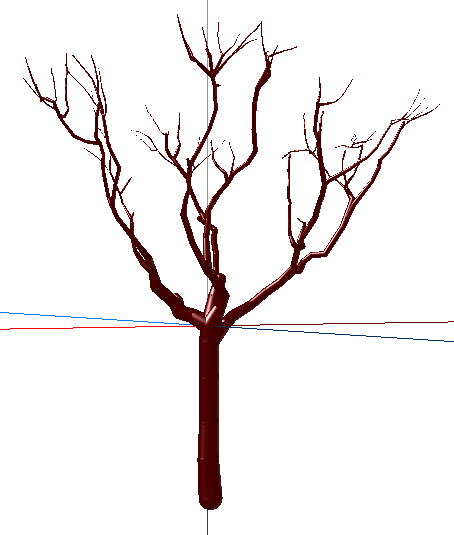
\includegraphics[height=6cm]{raffine.png}}\hspace{4em}
	\caption{三种计算半径方法效果对比}
	\label{fig:radius}
\end{figure}

对于骨架长度的估计,基于规则的生成则并不那么具有实践性,因为树木枝干的长度往往并不像半径那样
随着父子关系而递减。相反地,它地规则往往要复杂许多,而且并没有统一的规则。基于此考虑,本文并
没有对基于规则的长度估计进行实践,而是直接用与半径类似的方法,根据已拟合出的直线,试图从统计
的角度对其枝条长度做出合理的估计。一个直观而可行的方法,是将当前节点与所有该方向邻域的点的连线向量
投影到拟合出的直线方向向量上,这个投影的平均值的2倍,则可以估计为该方向子枝的长度。本文也给出了
子枝长度估计的伪代码,列在了算法\ref{alg:length}中。

\begin{algorithm}[H]
	\caption{子枝长度抽取}
	\label{alg:length}
	\begin{algorithmic}[1] 
		\Require 拟合出的当前子枝方向向量$L$,父节点$N$
		\Require 当前子枝的点集$\mathbb{S}$
		\Ensure 当前子枝长度$L$
		\State 初始化父节点到邻域点的向量投影长度之和$D_{sum}=0$
		\ForAll{空间点$P \in \mathbb{S}$}
		\State 父节点到$P$的向量$Dir=P$.Position-$N$.Position
		\State $Dir$在$L$上的投影距离$D_{sum}+=$CalculateProjectionLength$(Dir, L)$
		\EndFor
		\State 平均距离$D_{avg}=D_{sum}/\mathbb{S}.Count$
		\State 子枝长度$L=D_{avg}*2$
		\State \Return $L$
	\end{algorithmic}
\end{algorithm}

%---------------------------------轻量化-----------------------------------
\clearpage
\section{基于枝干合并的轻量化处理}
\label{sec:branchcombine}
用基于多方向迭代与步长探索得到的三维树木骨架通常是很细致和准确的,尽管它相对于
用3DSMAX等建模工具手工建模得到的面片模型已经大大的轻量化了。但是如果应用是用于
大规模的树木建模,那么我们有必要根据应用需求进一步进行轻量化处理。

\subsection{L-System的尝试}
\label{subsec:lsystem}

\subsubsection{L-System简介}
L-System是一种并行的重写系统和正规语法,
它的结构可以用可以定义为一个3元组:\\
\[\mathbf{M} = (V, \omega, P)\]
其中:\\
\begin{itemize}
	\item $\mathbf{V}$(字母表) 表示可以被替代的字符的集合。
	\item $\mathbf{\omega}$(初始串) 表示L-System的初始状态。
	\item $\mathbf{P}$(规则集合) 表示一系列的衍生规则。
\end{itemize}
L-System可以根据这三个组成部分的不同而递归地产生形态各异的字符串。
由于L-System具有递归生长的特性,因此我们可以用L-System规则来表达一个具有自相似形态
或者分形结构的物体,比如本文所研究的对象\raisebox{0.5mm}{------}树木。

\subsubsection{树木模型的参数化L-System规则抽取}
球面海龟几何的提出,用参数化的L-System规则描述了树木的结构信息。在球面海龟几何中,
节点的空间几何信息用4个量(长度$l$、半径$r$、父子枝夹角$\theta$和水平转角$\phi$)
和4个扩展符号(+、-、\&、$\wedge$)来表示:
\begin{itemize}
	\item $+(l)$	表示以当前位置为起点,在当前方向上前进$l$单位个长度
	\item $!(r)$	表示设置当前节点半径为$r$
	\item $\&(\theta)$	表示设置父子枝夹角为$\theta$
	\item $\wedge(\phi)$	设置水平偏角为$\phi$
\end{itemize}
在球面海龟几何中,将每个骨架节点生成一条参数化的L-System规则,形如:\\
\begin{equation} \label{eq:turtle}
N(l,r) \rightarrow \&(\theta_0)\wedge(\phi_0)!(r) + (l)S_0(l*a_0,r*b_0)...\&(\theta_n)\wedge(\phi_n)!(r) + (l)S_n(l*a_n,r*b_n)
\end{equation}

其中N表示当前枝条,$S_0~S_n$表示当前枝条的n个子枝条,$a_i和b_i$分别表示第i个子枝条
与当前枝条的长度比和半径比,$\theta_i和\phi_i$分别表示第i个子枝条与当前枝条的空间
夹角和水平偏角。

\subsubsection{使用L-System进行树木轻量化建模遇到的问题}
在用参数化L-System进行树木轻量化建模时,在进行规则归纳时,有个难以克服的问题。考虑
将规则\ref{eq:turtle}中的$a_0$换成$a_0'$,则规则变成一个完全不同的规则。这意味着对于
两个分支规则,这两个规则中的子枝的长度,半径,转交,偏角等必须完全相等才能归纳为同
一个规则。而对于自然界中形态结构复杂的树木,每个分支规则几乎不可能完全等同于另一个
规则。

对上面的问题有一种解决方法就是将参数区间化,将属于同一区间的参数的值视为相同。比如
我们可以将父子枝间的转角分为18个区间,每个区间的大小为10度。但是经过分析就可以察觉,
这并没有从根本上解决这个问题。假设我们将这4个变量都各自划分为10个区间,那么规则总数
最多可以有10000个,而且在这种情况下,两个规律相同的几率也是非常小的。如果我们将分区
数量减少,则又有可能将本来差异比较大的规则归纳为一个规则,不符合真实感的要求。

所以,经过分析,这种用参数化L-System进行树木轻量化建模的方法并不适用于从骨架中去抽取
规则,而是适用于反向地用其描述的规则去产生一棵树,如台湾学者戴文凯就对单棵树的L-System
规则进行随机扰动而轻量化的建模出了整片森林。

\subsection{树木轻量化?枝干合并!}
\label{subsec:branchmerge}
用L-System的方法抽取规则所产生的问题,从本质上看,是由于自然界中的树木形态太复杂和多变。
与其从一个本就不规则生长的事物中去抽取规则,还不如直接地在其逻辑结构上进行一系列的轻量
化操作。本文提出了对已抽取的树木骨架中对视觉影响不大的部分进行合并的方法,从而在尽可能
保证模型的视觉效果的基础上,进一步地减小树木模型的体积,使得其能更广泛地应用到WebVR、WebGame
等各个领域。

树枝的结构其实只由核心的一些枝干组成,其他的枝干只是对其结构进行微调。所以在要求进一步轻量化
的前提下,本文提出了分别从纵向和横向对树枝进行合并的方法,以去掉一些只是起到微调作用的枝干。
这种方法在尽可能保证真实感不过多丢失的前提下对树枝进行简化操作,以适应更广泛的Web应用领域。

纵向合并表示从父到子,从根到页进行纵向递归式的合并。若当前节点与其父节点和子节点的夹角小于所设定
的阈值,那么则将该节点去掉,并将其子节点连接到其父节点。注意,若该节点的子节点数目不只一个,
那么我们不对它进行合并操作,因为将该节点的所有子节点加到该节点的父节点上去有违真实感。
图\ref{fig:vert}展示了树枝纵向合并过程。图\ref{fig:vert}(a)为输入的树枝骨架,并且当前节点
为\textbf{B},其父节点为\textbf{A},且只有唯一的子节点\textbf{C}。设合并角度阈值为$\alpha$,
假设\textbf{AB,BC}之间的夹角b小于合并阈值$\alpha$,那么将\textbf{B}剔除,并将\textbf{C}作为
\textbf{A}的子节点。同理,在图\ref{fig:vert}(b)中,若夹角c小于阈值$\alpha$,那么也将\textbf{AC}
和\textbf{CD}合并。在图\ref{fig:vert}(c)中,由于节点\textbf{D}有两个孩子,所以不对其进行合并
操作。

纵向合并算法的伪代码在算法\ref{alg:vertical}中给出。

\begin{figure}[H]
	\centering
	\subfloat[输入树枝骨架]{
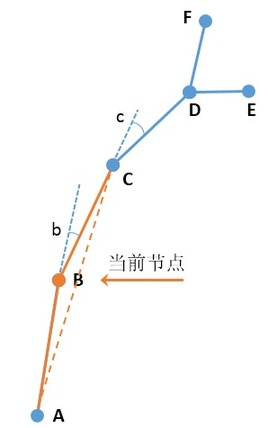
\includegraphics[height=5cm]{vert1.jpg}}
\hspace{4em}
	\subfloat[合并AB、BC]{
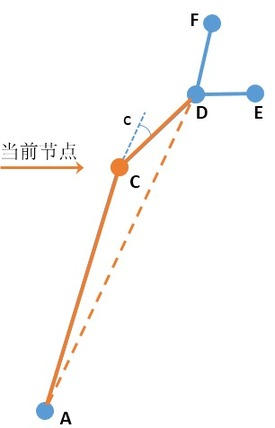
\includegraphics[height=5cm]{vert2.jpg}}
\hspace{4em}
	\subfloat[合并AC、CD]{
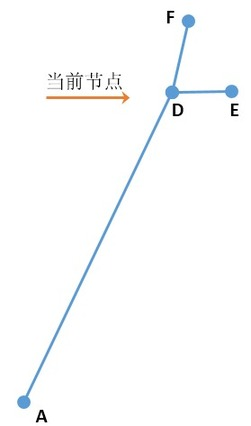
\includegraphics[height=5cm]{vert3.jpg}}
	\caption{树枝简化过程}
	\label{fig:vert}
\end{figure}

\begin{algorithm}[H]
	\caption{纵向合并枝干}
	\label{alg:vertical}
	\begin{algorithmic}[1] 
		%\Comment {根据纵向合并角度参数,以当前节点为发起点递归式地纵向合并枝干}
		\Require 纵向合并角度$\alpha$
		\Require 当前节点$N$
		\Ensure None
		\ForAll{节点$N'\in N.Children$}
		\While{$N'.ChildCount = 1$}
		\State $\vec{u} \gets N'.Position-N.Position$
		\State $\vec{v} \gets N''.Position-N'.Position$
		\State $\gamma \gets \cos^{-1}({\frac{\vec{u} \cdot \vec{v}}{|\vec{u}|\cdot|\vec{v}|}})$
		\If{$\gamma<\alpha$}
		\State $N.child \gets N.AddChild(N'')$
		\State $N.child \gets N.DeleteChild(N') $
		\EndIf
		\State $N' \gets N'.FirstChild$
		\EndWhile
		\EndFor
		\If{$N.ChildCount > 1$}
		\ForAll{节点$N'\in N.Children$}
		\State 以$N'$为当前节点递归调用该函数
		\EndFor
		\EndIf
	\end{algorithmic}
\end{algorithm}

横向合并指的是对叶子节点和与其夹角小于阈值的兄弟节点进行合并。之所以只对叶子节点进行合并,是
因为非叶子节点下面都有若干棵子树,若对它们进行合并,必须对它们下面的子树也进行合并。而合并子树
显然就使得真实感下降很大,因为这不只是局部微调,而是若干子树的变动。横向合并的伪代码在算法\ref{alg:hori}中
给出。

\begin{algorithm}[H]
	\caption{横向合并枝干}
	\label{alg:hori}
	\begin{algorithmic}[1] 
	\Require 初始化横向合并角度$\beta$
	\Require 设定当前节点$N$
	\Ensure None
	\ForAll{节点对$P\in N.Children$}
		\State $N_1 \gets P.FirstNode$
		\State $N_2 \gets P.SecondNode$
		\If{$N_1.ChildCount = 0 \wedge N_2.ChildCount = 0$}
			\State $\vec{u} \gets N_1.Position - N.Position$
			\State $\vec{v} \gets N_2.Position - N.Position$
			\State $\gamma \gets \cos^{-1}({\frac{\vec{u} \cdot \vec{v}}{|\vec{u}|\cdot|\vec{v}|}})$
			\If{$\gamma<\beta$}
				\State $New\ Node\ N'$
				\State $N'.Position \gets (N_1.Position+N_2.Position)/2$
				\State $N'.Radius \gets max(N_1.Radius,N_2.Radius)$
				\State $N.child \gets N.DeleteChild(N_1)$
				\State $N.child \gets N.DeleteChild(N_2)$
				\State $N.child \gets N.AddChild(N')$
				\State 退出循环并以当前节点N重新调用该函数
			\EndIf
		\EndIf
	\EndFor
	\ForAll{节点$P\in N.Children$}
		\State 以P为当前节点递归调用该函数
	\EndFor
\end{algorithmic}
\end{algorithm}

纵向合并和横向合并单独使用时都具有很大的局限性,因为纵向合并只能对具有单个孩子并且没有
兄弟的节点进行纵向递归地调用,而横向合并又只能对叶子节点进行兄弟级别的合并。但是将两种
合并方法联合使用,将可以从整体上对树木进行微调操作,图\ref{fig:combine}对这一想法进行了
演示。\ref{fig:combine}(a)中经过纵向的\textbf{AC,CD}合并得到\ref{fig:combine}(b)。
\ref{fig:combine}(b)中由于\textbf{D}有两个子节点,无法进行纵向合并,所以考虑进行横向
合并\textbf{DE,DF},并得到\ref{fig:combine}(c)。最后进行一次纵向合并得到\ref{fig:combine}(d)。

\begin{figure}[H]
	\centering
	\subfloat[输入枝干骨架]{
	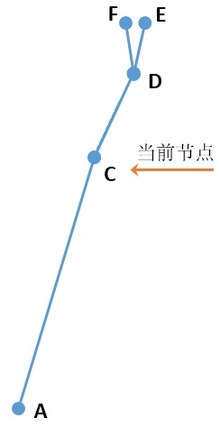
\includegraphics[height=3cm]{comb1.jpg}}
	\hspace{4em}
	\subfloat[纵向合并AC,CD]{
	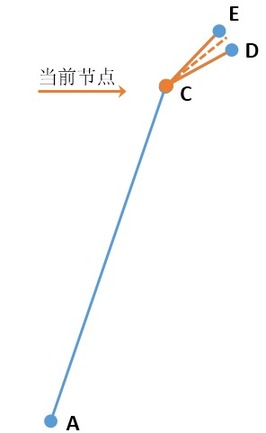
\includegraphics[height=3cm]{comb2.jpg}}
	\hspace{4em}
	\subfloat[横向合并DE,DF]{
	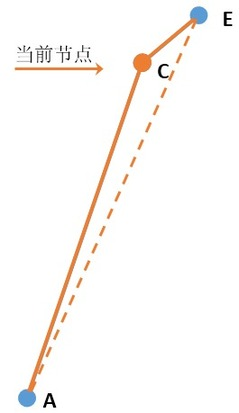
\includegraphics[height=3cm]{comb3.jpg}}
	\hspace{4em}
	\subfloat[纵向合并AD,DE]{
	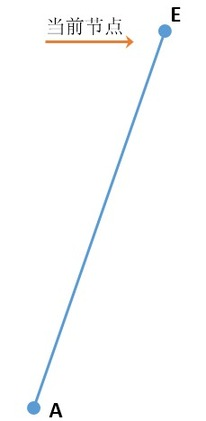
\includegraphics[height=3cm]{comb4.jpg}}
	\caption{联合使用纵向和横向合并}
	\label{fig:combine}
\end{figure}

%---------------------------------质量评估----------------------------------
\section{建模还原度}
\label{sec:qualityevaluation}
对于一个通过建模获得的树木模型,如果没有一个客观的量化评价指标,就无法从客观的角度
反馈树木模型的还原度和各个步骤算法的可行性。对于本文的基于图像序列的树木建模方法,
建模的输入是在自然环境下拍摄的树木图片序列,输出是三维的骨架模型。因此,判断三维模型
和投影照片的相似程度是评价建模质量的核心。然而,大多数基于图像的树木建模论文\cite{quanlong,
tanping,lichuan,tanping2,liu}只给出了输入图片和建模结果在少量角度的渲染效果,试图让
观察者从肉眼观察其相似度。但是这种方法是主观的,因观察者的不同可能会有不同的评价结果,
这显然不是一个好的评价方法。

为了客观、量化地评价基于图像序列的建模质量,本文提出了一套完整的评价方法。然而,仅仅凭借照片
无法完全表达出其所在环境的信息,比如环境光照,因为遮挡而产生的阴影信息等,因此本文的评价
方法将不针对模型的纹理和颜色信息,仅仅对模型的几何信息和照片中的几何信息的匹配程度进行量化
分析。

设树木模型$M$由$n$张从不同角度拍摄的同一棵树的图片序列$I_1\sim I_n$,经过基于图像的三维重建,
骨架抽取的方法进行建模所获得。那么模型$M$的建模还原度$\mathbb{Q}$定义如下:\\
\begin{definition}
	\[\mathbb{Q}=\mathbf{I}\cdot\mathbf{R_{3d}}\cdot\mathbf{R_s}\]
\end{definition}

建模还原度$\mathbb{Q}$的取值范围为$[0,1]$,0表示没有还原出任何树木几何信息,1表示准确还原出
整棵树木的几何信息。

本文将建模还原度$\mathbb{Q}$考虑由3个部分组成,为此也引入了三个新的概念:图片序列信息量$\mathbf{I}$,
三维重建还原度$\mathbf{R_{3d}}$,以及骨架抽取还原度$\mathbf{R_s}$。这三个分量的取值范围都为$[0,1]$,它们
的乘积即为总的建模还原度$\mathbb{Q}$。后续小节会详述这三个分量。

\subsection{图像序列信息量}
当实地对树木进行多角度拍摄时,拍摄者将基于不同的水平角度对树木进行全方位的拍摄,以便将整棵树的
信息尽可能多的携带进图像序列中。然而,从客观上来看,怎么样的图片序列才更加完整的表达了整棵树的
几何特征?为了从客观和量化的角度给出树木图像序列所携带的树木信息的多少,本文引入了图像序列信息量的概念。

那么,到底怎样的图片序列携带的信息量更大呢?从拍摄过程分析,如果想要得到一棵完整的树木信息,那么
需要绕着一棵树一圈进行密集地拍摄。这里的一圈,用数学化的表示,就是$360^\circ$,如果只是绕半圈进行
拍摄,那么所得到的图片序列表达的树木信息必定是不完整的,所以角度对信息量有着很大的贡献。另一方面,
如果每隔$60^\circ$进行一次拍摄,和每隔$30^\circ$进行一次拍摄,在它们都绕圈拍摄的前提下,后者的图片序列所
含信息量必然更大。再进一步思考,如果我隔$360^\circ,180^\circ,90^\circ,..., 1^\circ$进行拍摄呢?那么后一次拍摄所得的图
片序列相比前一次的图片序列信息量的增长是相同的吗?答案是否定的,因为当图片很少时,三维重建的结果也不好,
这时增加图片数量是能够很大程度上改观三维重建的重量的,因此此时的信息量增长速度快。
但是在拍摄已经比较密集的情况下,后一次拍摄所增加的信息量必定只是一些细节的信息,所以,信息量增长的速率应该变小。
并且一个信息量大的图片序列应该满足以下三个要求:\\
\begin{itemize}
	\item \textbf{图片数量多}: 图片数量多也就意味着拍摄角度多,因为一张图片代表着一个角度。
	\item \textbf{角度跨度大}: 跨度大指需要对树木进行全方位的拍摄。
	\item \textbf{角度分布均匀}: 若图片只是密集的集中在一个角度区间,就算图片再多,也无法完整地表达整
								  棵树的信息,所以若在角度多和跨度大的情况下还满足分布均匀,那么就能很完整
								  地携带树木的信息。
\end{itemize}

由于从平面的2D图像很难得到其空间角度拍摄情况,因此在这里我们简化其定义,将关注点放在图片数量上来,对于
图片跨度和角度的均匀分布,我们默认拍摄者在拍摄过程中采用均匀的角度偏差来进行$360^\circ$的拍摄。

根据以上的分析,本文给出了图像序列信息量的数学定义如下:\\
\begin{definition}
	\[ \mathbf{I}=1-(\frac{a}{b})^n \]
\end{definition}

其中,图片序列信息量$\mathbf{I}$的取值范围为$[0,1]$。当$\mathbf{I}=0$时表示图片序列并不包含树木信息,
当$\mathbf{I}=1$时表示图片序列能完全表达空间树木的几何信息。$a,b$都是正数且$a<b$,具体数值需要对不同树木
进行实验之后才能得到。尽管$a$和$b$因树木特点不同而不同,但是它始终满足前文提出的信息量增长速度的特点,
即先快后慢。

\subsection{三维重建还原度}
对于一个给定的图片序列,所用三维重建方法所得到的点云模型的与实际的树木在几何形状上的相似度如何,由三维重建
还原度$\mathbf{R_{3d}}$来定义。注意,实际树木的几何信息被记录在输入的图像序列中,所以想要计算点云模型和实际树木
的相似度,就需要对点云模型和图片序列进行比较。然而对于三维的点云信息和二维的图片信息,无法进行直接地比较。一个
比较直观的想法,是对三维的点云进行投影,投影的角度由三维重建过程中的照相机几何标定步骤给出。

由于不考虑模型纹理和颜色信息,在空间点被投影到平面以后,只关注其是否在对应角度图片的树木轮廓内。所以对输入的树木
图片序列,需要先获得其轮廓图,并将其转化为二值图像。树木上的点值为1,而树木外的点值为0。对于每一个点云模型中的点,
按对应角度投影,获得其在对应图片上的坐标值,并且在其二值图像上确定其值,若为1,则表明匹配成功,否则匹配失败。最后
统计出匹配成功的总的比例,作为三维重建的还原度。

根据以上分析,本文给出三维重建还原度的数学定义式:\\
\begin{definition}
	\[ \mathbf{R_{3d}}=\frac{1}{n}\sum_{i=1}^n \frac{P_i}{P_i+O_i}\]
\end{definition}

上式中的$n$表示图像的数量,$P_i$表示点云模型投影到第$i$张图片上在树木轮廓中的点的数量,$O_i$表示点云模型投影到第
$i$张图像上在树木轮廓外的点的数量,因此$P_i+O_i$自然就表示点云模型中点的总数量。$\frac{P_i}{P_i+O_i}$表示点云投影到
第i张图片上的击中率。最后对每张图像的击中率求平均,作为总的三维重建的还原度。其值区间为$[0,1]$。

\subsection{骨架抽取还原度}
骨架抽取是基于三维点云模型进行的,因此计算骨架抽取的还原度的输入是重建出的点云模型和抽取出的骨架模型。由于点云模型是
三维的点的集合,而抽取出的骨架模型却是一个记录着树形结构的逻辑信息,它们无法进行直接的比较。本文采取的做法是将骨架的
树形逻辑信息用圆台和球进行堆叠从而将其转化为三维的表示。

具体的做法是对骨架中的每个节点,根据其半径构造出一个球体。然后对于每个父子关系,用一个圆台来表示其枝干,圆台的底半径
等于父节点的半径,圆台的顶半径等于子节点的半径。然后对于每个点云模型中的点,用数学公式判断其是否存在于骨架的三维表示中
的球体或圆台中,如果存在,则表示匹配成功,否则表示匹配失败。最后用成功点数与总点数的比值来表示骨架抽取的还原度。定义如下:\\
\begin{definition}
	\[ \mathbf{R_s}=\frac{S}{N} \]
\end{definition}

其中$S$表示匹配成功的点数,而$N$表示点云模型的总点数。$\mathbf{R_s}$的值区间为$[0,1]$。

注意,若用经过枝干合并轻量化处理的骨架进行骨架抽取还原度计算,其值必定会比直接从点云中抽取出来的模型要小,因为模型经过
简化后,与原点云模型的匹配度也必将降低。本文的目标只是尽可能在还原度降低不多的情况下,对骨架进行尽可能多的轻量化。

\subsection{建模还原度计算}
将图片序列信息量$\mathbf{I}$、三维重建还原度$\mathbf{R_{3d}}$和骨架抽取还原度$\mathbf{R_s}$代入建模还原度$\mathbb{Q}$
的定义式中,可以得到建模还原度的计算式:\\
\begin{equation}
	\mathbb{Q}= (1-(\frac{a}{b})^n)\cdot \frac{1}{n}\sum_{i=1}^n \frac{P_i}{P_i+O_i} \cdot \frac{S}{N}
\end{equation}

\clearpage
\section{本章小节}
\label{sec:conclusion}
本章具体阐述了基于图像树木轻量化建模所涉及的一些算法。

首先介绍了光流法的由来,并且分析了LK光流法的思想和特点,然后介绍了基于图像金字塔的PyrLK光流法,这种方法用图像金字塔这种多
分辨率图像层来克服图像中的大块运动,是LK光流法的一种优化与实现。接着提出了改进的PyrLK光流法,该算法把PyrLK的局部平移假设
扩展到了局部仿射变换假设,并且加入了特征反向追踪,以提高算法鲁棒性,实现了高精度的匹配。

三维体素泛洪是计算机图形学中二维像素泛洪的扩展,它将三维体素按洪水泛滥一般进行空间的扩展。本文利用三维体素泛洪实现了节点
对邻域的探索,并在该邻域的范围内对方向进行分割,将每个分割方向上的点集根据最小二乘法进行拟合,得出该方向上骨架具体的直线方程。
然后根据点集内点到对应直线方程的距离大小,算出该骨架的半径大小。从而得到具有半径信息的骨架结构。

在得到骨架结构后,为了迎合轻量化的应用,本文对其进行轻量化操作。本文首先对传统的轻量化方法L-System进行了尝试,运用参数化
的L-System规则进行规则抽取,但是由于现实中树木的复杂性与不规则性,抽取出来的规则太多,以至于违背了轻量化的原则。于是本文
提出了基于枝干合并的轻量化方法,分别从纵向和横向对树木枝干进行合并,以达到轻量化的目标。

本章的最后,本文还提出了基于图像树木轻量化建模的质量评价方法。提出了建模还原度的概念,它包含了三个子项:图像序列信息量、
三维重建还原度以及骨架抽取还原度。它们分别代表了图像序列对真实树木的信息携带量、点云模型和图像序列的匹配度和骨架模型与点云模型的匹配度。
本文对这三个子项的由来和计算方法都进行了阐述,并将它们融合给出了建模还原度的计算式。
